\subsection{Frontend}

Como referido anteriormente, o módulo de \textit{Frontend} encontra-se exclusivamente dedicado à visualização e interação com os elementos de negócio, tendo como principal objetivo a implementação de uma interface de utilização simples e intuitiva. Para alcançar este propósito, recorreu-se a ferramentas de design, nomeadamente o \textit{Figma}, que possibilitaram a prototipagem e a definição estruturada da interface antes da sua implementação final.

\subsubsection{React}

O \textit{React} consiste numa biblioteca de \textit{JavaScript} concebida para a criação de \textit{Single Page Applications} (aplicações de página única). A sua arquitetura baseia-se no conceito de componentes, que correspondem a unidades de código modulares, reutilizáveis e personalizáveis, responsáveis por encapsular a interface, o comportamento e o estilo de forma estruturada.

Um dos aspetos centrais do React é a utilização do \textit{Virtual DOM}, que permite atualizar de forma eficiente a interface em função das alterações de estado, evitando manipulações diretas do DOM real, que são mais custosas em termos de desempenho. Esta abordagem declarativa contribui para a criação de interfaces interativas, escaláveis e de fácil manutenção, adequadas a projetos que exigem dinamismo e modularidade.


\subsubsection{Paginas Estáticas}

Por especificação do cliente existia um importante foco nas páginas estáticas do \textit{website}. Era exigido a criação de páginas que funcionacem com um \textit{elevator pitch} para cada um dos atores do negócio.

\begin{figure}[h!tbp]
    \centering
    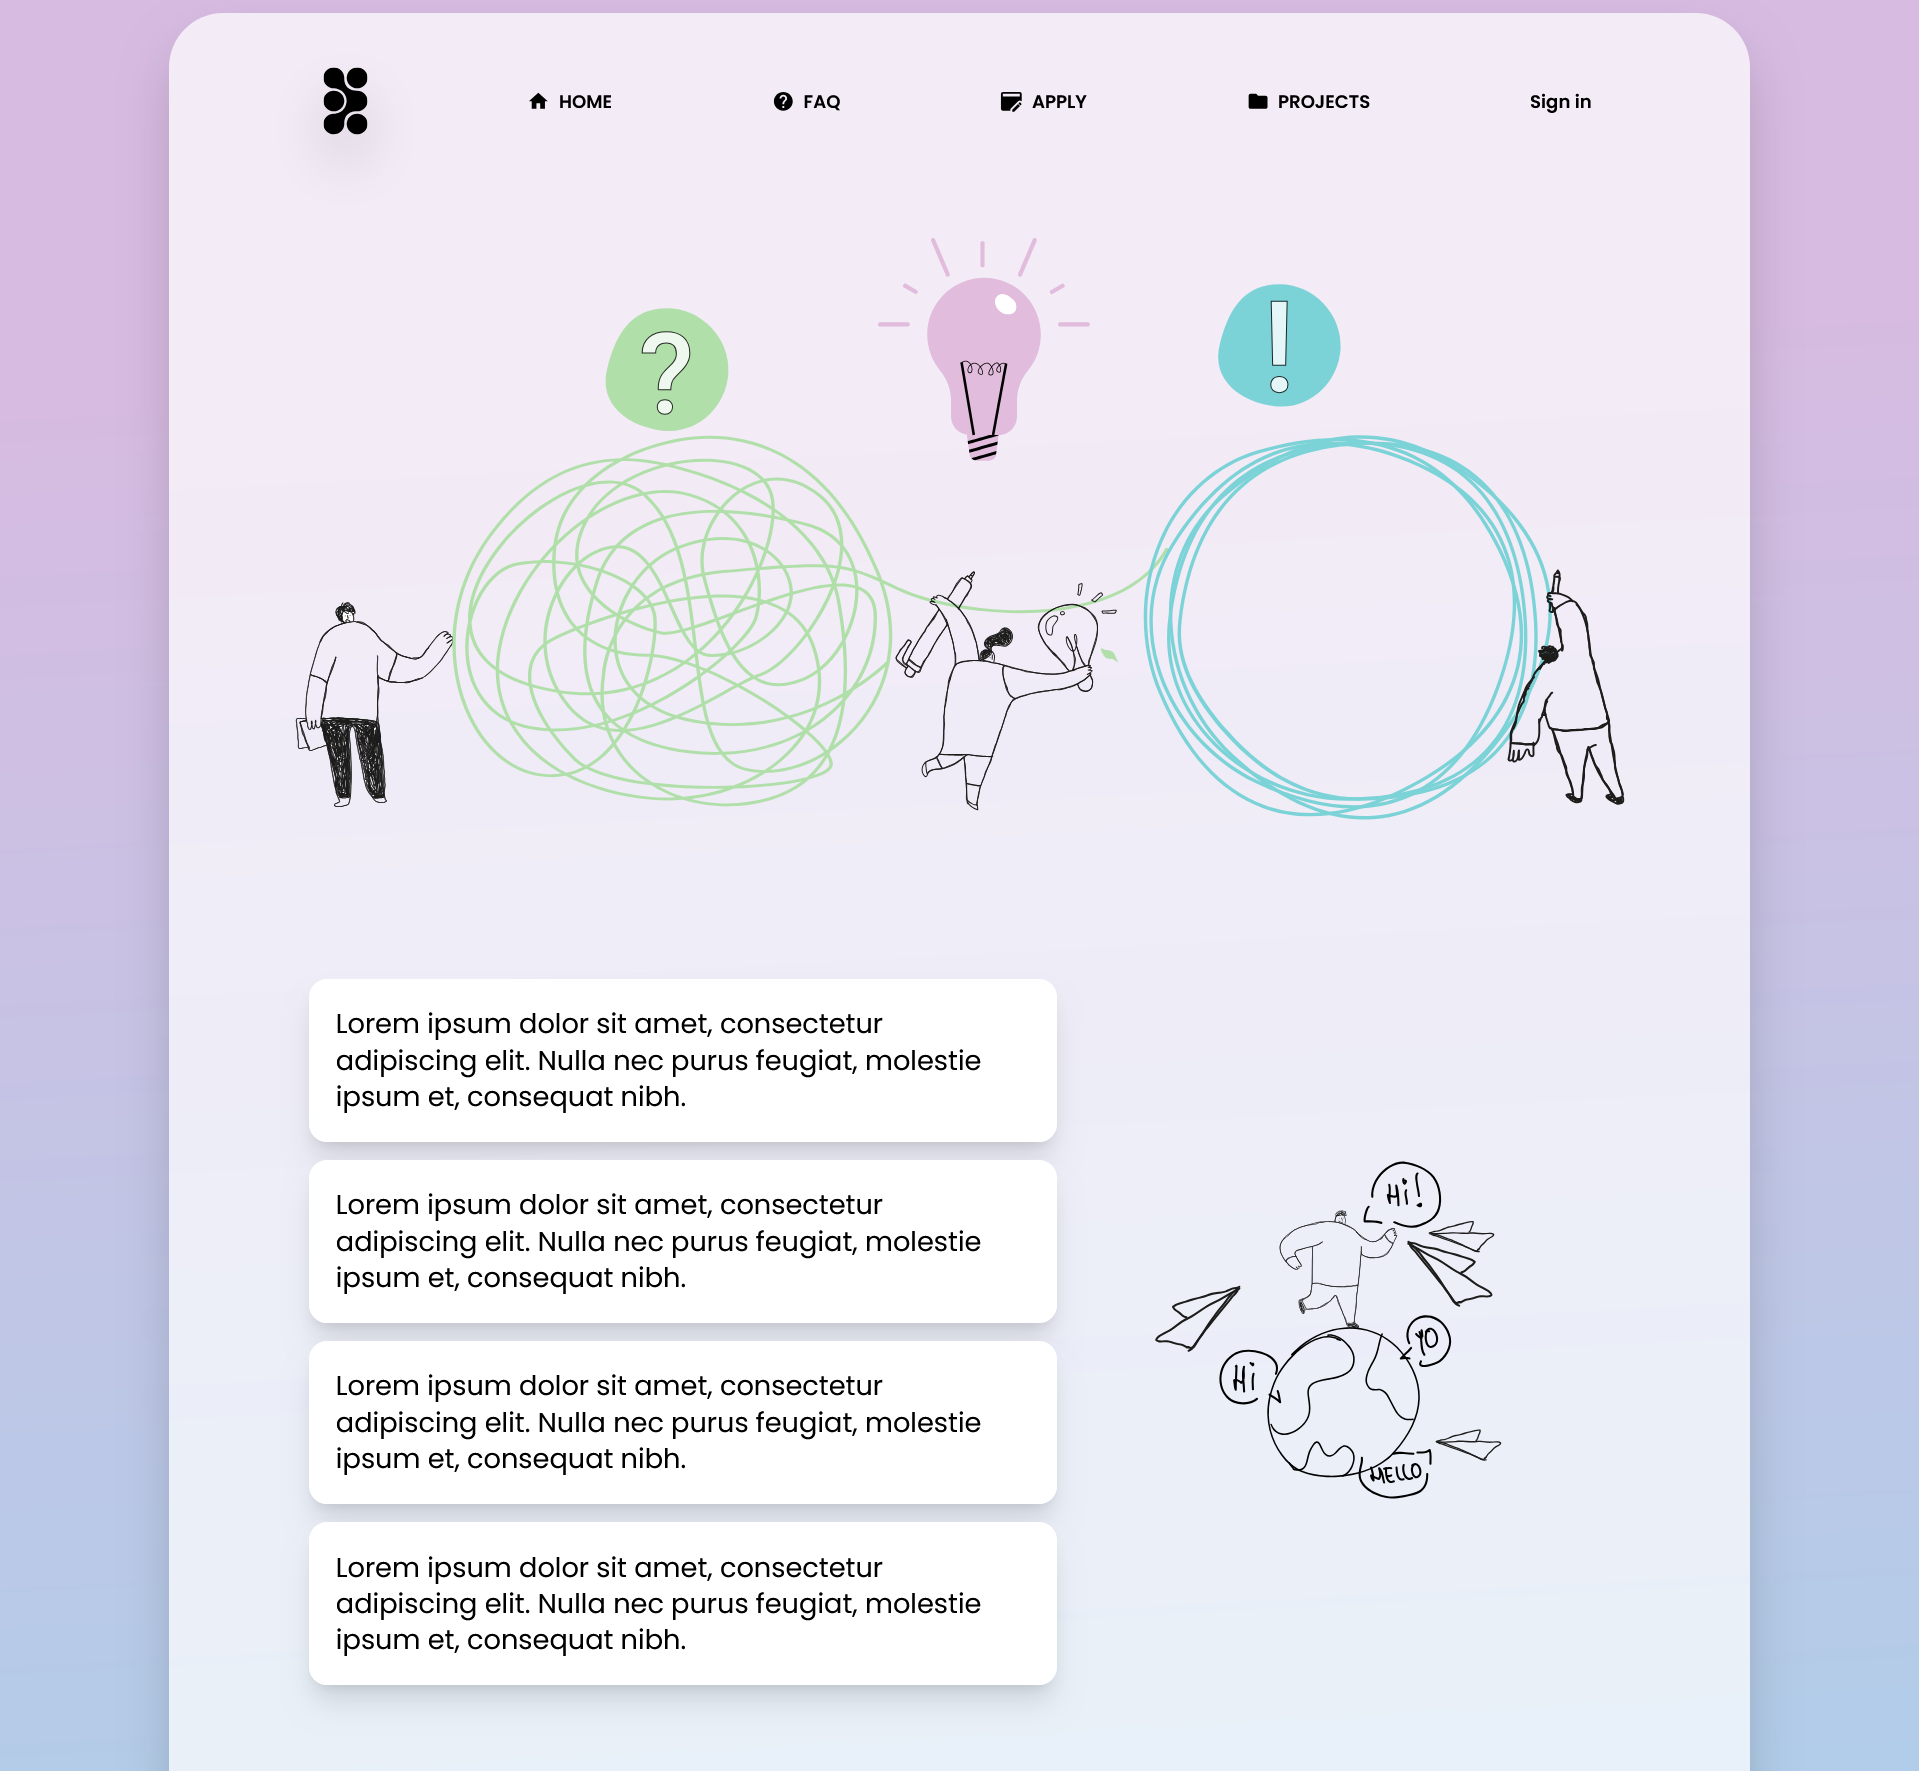
\includegraphics[width=0.7\linewidth]{capitulos/cap4-implementacao/assets/frontend/blende-website1.png}
    \caption{Pagina \textit{Elevator Pitch} de estudante - parte 1}
    \label{fig:frontend-student-page}
\end{figure}

\begin{figure}[h!tbp]
    \centering
    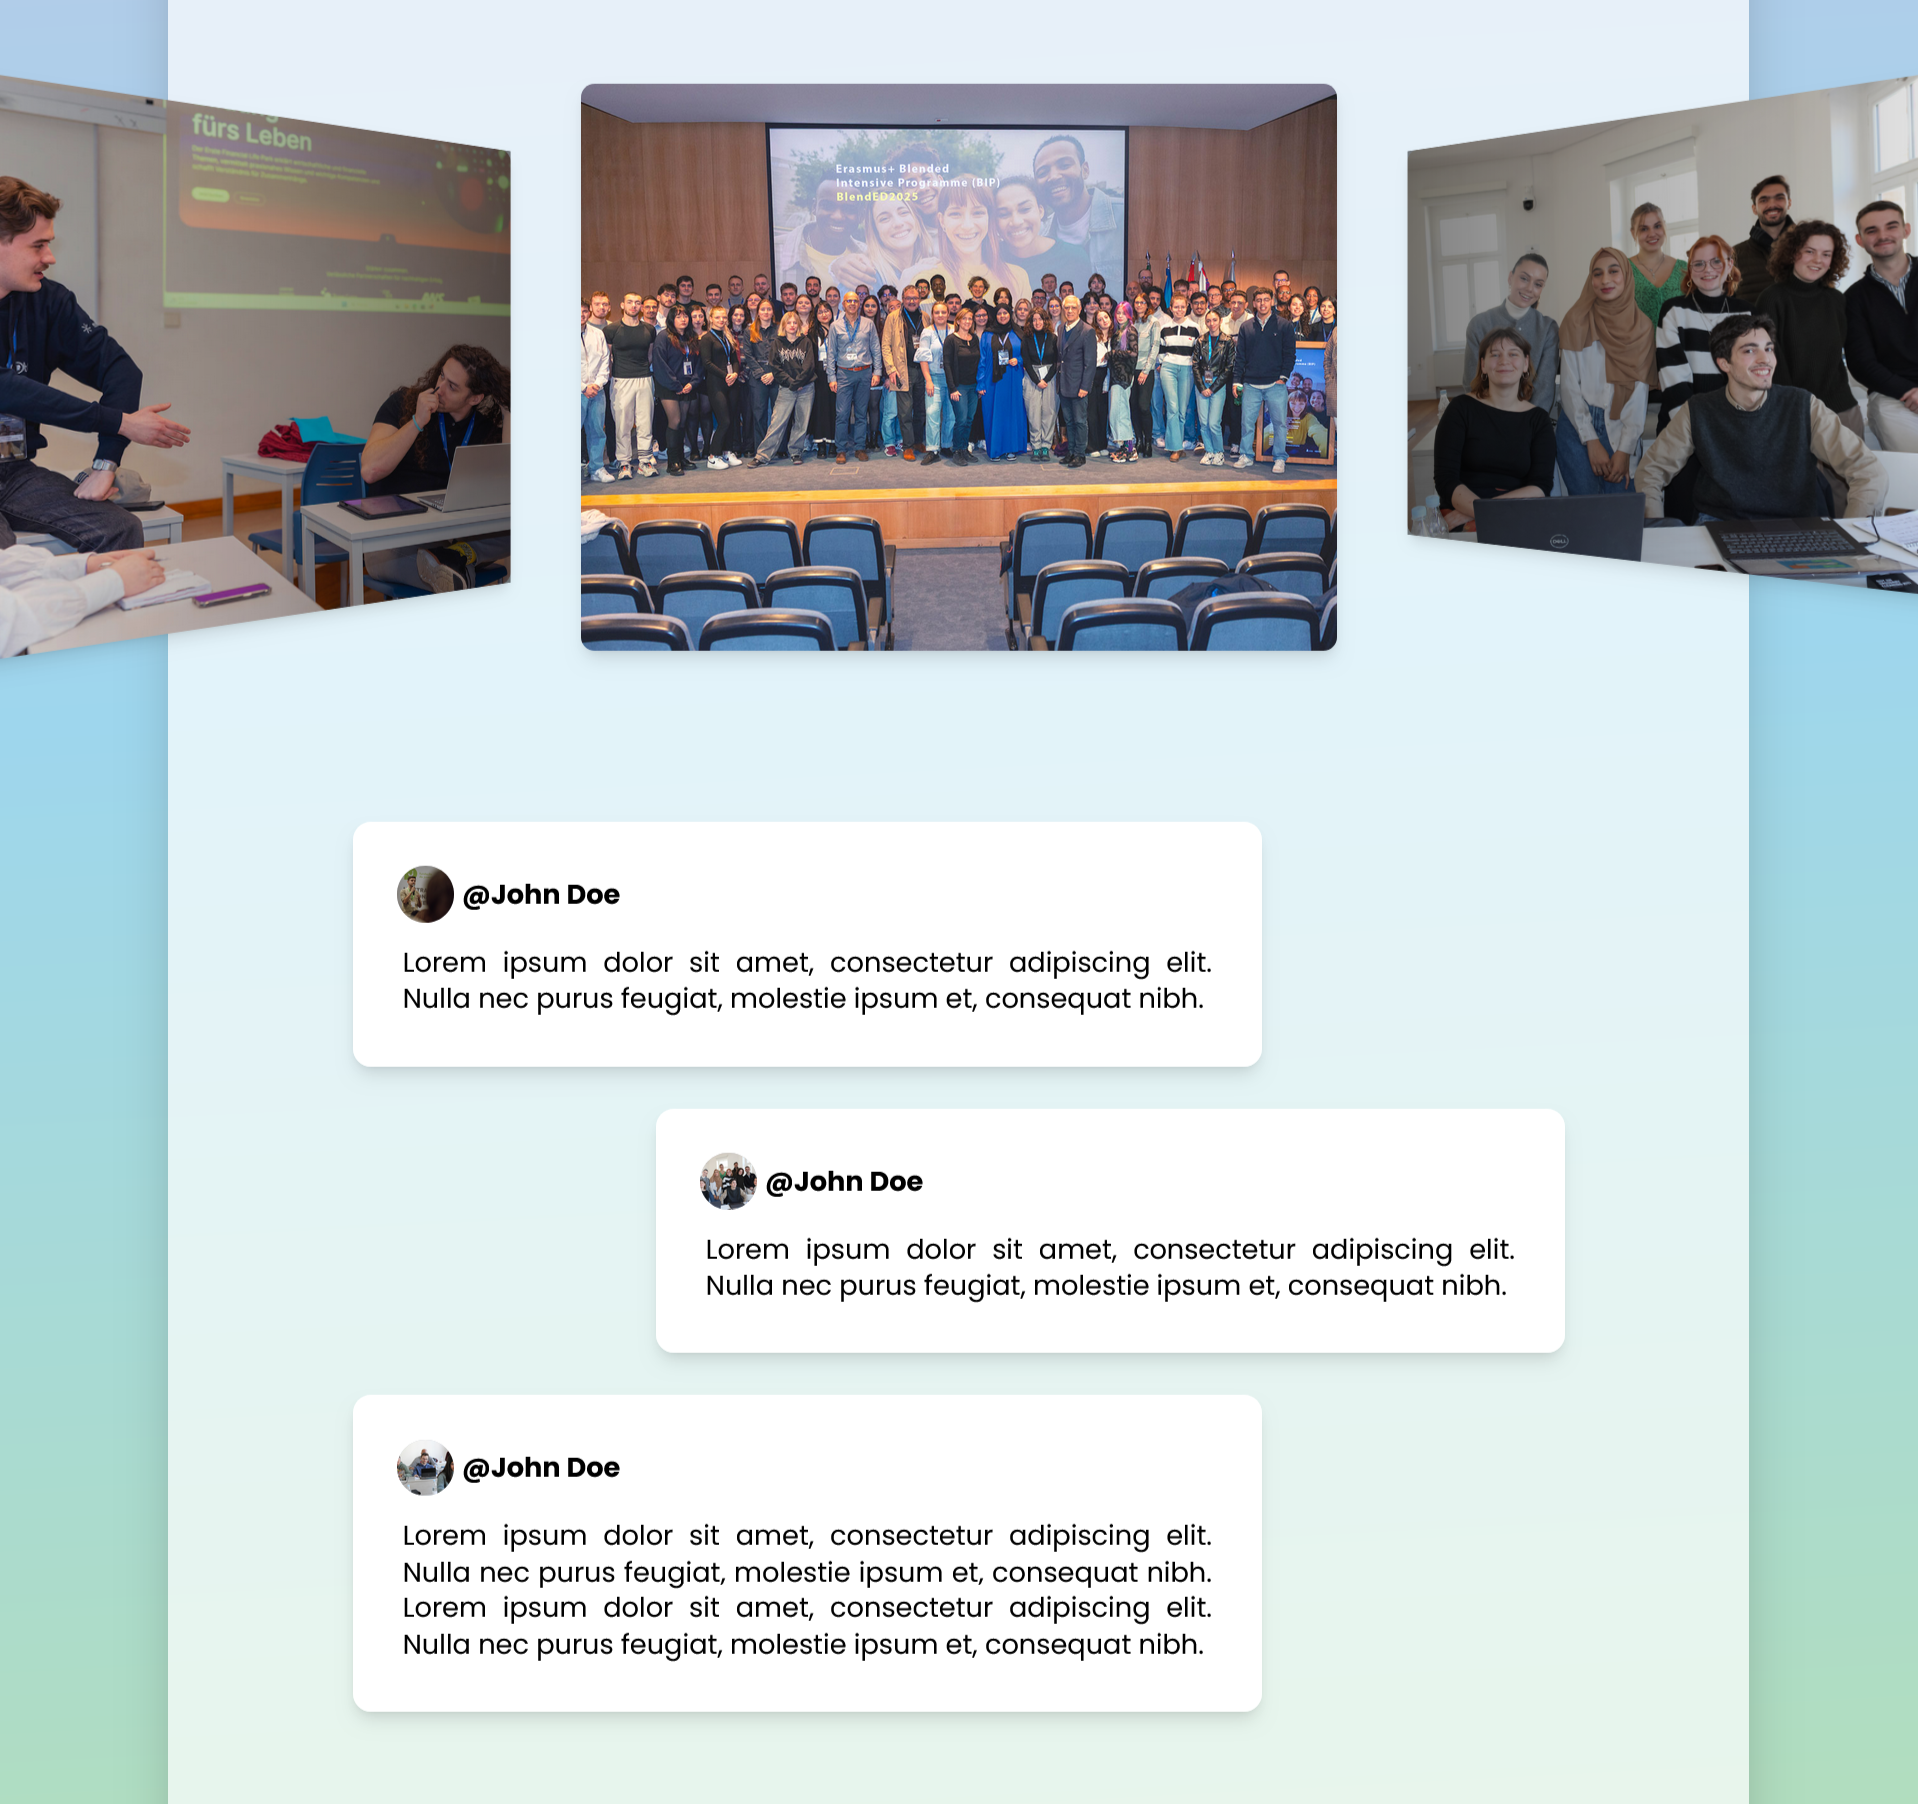
\includegraphics[width=0.7\linewidth]{capitulos/cap4-implementacao/assets/frontend/blende-website2.png}
    \caption{Pagina \textit{Elevator Pitch} de estudante - parte 2}
    \label{fig:frontend-student-page}
\end{figure}

\begin{figure}[h!tbp]
    \centering
    
\includegraphics[width=0.7\linewidth]{capitulos/cap4-implementacao/assets/frontend/blende-website3.png}
    \caption{Pagina \textit{Elevator Pitch} de estudante - parte 3}
    \label{fig:frontend-student-page}
\end{figure}

Para manter o efeito vidro + background com grandiente de cores foi implementado um componente \textit{wrapper} para todas as paginas do website. Na listagem \ref{lst:frontend-LandingPageContainer} é possivel ver essa implementação.

\begin{lstlisting}[caption={Função LandingPageContainer}, label={lst:frontend-LandingPageContainer}]
interface LandingPageContainerProps extends React.HTMLAttributes<HTMLDivElement> {
	className?: string;
    children?: React.ReactNode;
}

const LandingPageContainer = (props: LandingPageContainerProps) => {
    return (
        <div style={{paddingBlock:"12px", paddingInline:"10px"}} className="w-screen min-h-screen
            	 bg-gradient-to-b [background:linear-gradient(177deg,#D7BBE1_7%,#9ED6ED_45.52%,#CDE87B_95.32%)]
            	flex justify-center box-border
				px-20 py-2.5 overflow-x-hidden"
		>
			<div
				style={{ padding: "15px", borderRadius: "48px", gap: "12px", scrollSnapType: "y mandatory" }}
				className="w-full sm:w-full lg:w-4xl xl:w-10/12
            		p-10 rounded-28 shadow-2xl
            		bg-white/70 backdrop-blur-3xl box-border
					snap-y scroll"
			>
				{props.children}
			</div>
		</div>
    );
};
\end{lstlisting}

\subsubsection{Pagina de Visualização de Projetos}

A pagina de visualização de projetos era um dos elementos de maior importancia. Esta permite qualquer visitante do website visualizar os projetos que estão a ser realizados. A listagem \ref{lst:frontend-ProjectLibraryPage} permite entender a implementação desta pagina. Esta utiliza elementos essenciais do \textit{React}, como \lstinline|useState| e \lstinline|useEffect| que, respetivamente, permite 

\begin{figure}[h!tbp]
    \centering
    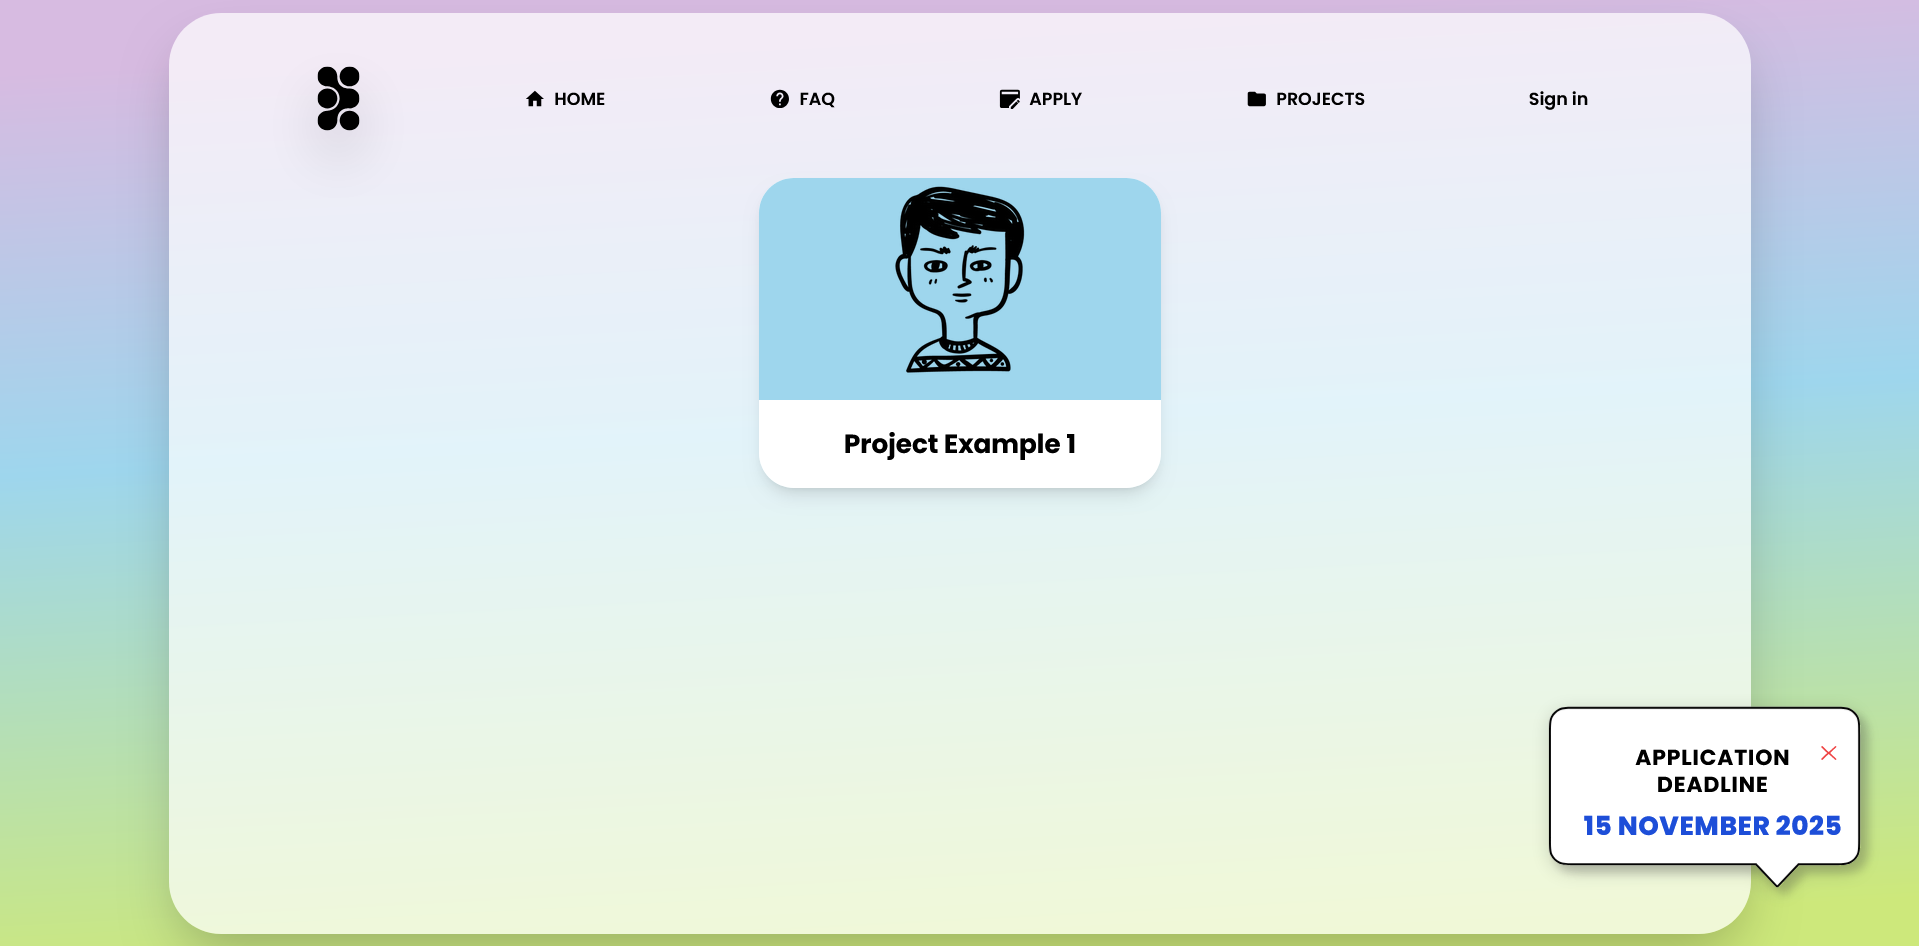
\includegraphics[width=\linewidth]{capitulos/cap4-implementacao/assets/frontend/blended-project-page.png}
    \caption{Pagina de visualização de projetos}
    \label{fig:frontend-project-page}
\end{figure}

\begin{lstlisting}[caption={Função ProjectLibraryPage}, label={lst:frontend-ProjectLibraryPage}]
const ProjectLibraryPage = () => {
  const projectService = new ProjectService();
  const [projects, setProjects] = useState<Project[]>([]);

  const fetchProjects = async () => {
    let req = await projectService.getAll();
    if (req.status > 300) {
      console.error(req.statusText);
      return;
    }
    setProjects(req.data.projects);
  };

  useEffect(() => {
    fetchProjects();
  }, []);

  return (
    <LandingPageContainer>
      <NavbarComponent />
      <div className="px-1">
        <div className="flex flex-wrap justify-center w-full gap-8 gap-y-8">
          {projects.map((project) => (
            <ProjectContainer project={project} key={project.id} />
          ))}
        </div>
      </div>
    </LandingPageContainer>
  );
};
\end{lstlisting}